\section{Experimentación}
Los primeros dos experimentos que veremos, se centran en el tiempo de ejecución de los procesos. Dichos experimentos tienen como finalidad estudiar como influye la cantidad de frames del video y la cantidad de frames a generar en el tiempo de ejecución, y si un video con mucho movimiento implica mayor tiempo de procesamiento que uno estático.\\

\subsection{Experimentación Temporal}

Como video de prueba, utilizamos una escena de un partido de futbol donde hay gran cantidad de movimiento y un video cuyos frames son todos blancos.\\

En el primer experimento medimos el tiempo de generación de frames aumentando en cada medición la cantidad de frames a generar en el video de futbol.

%grafico donde la cantidad de frames a generar aumenta
\begin{wrapfigure}{r}{0.6\textwidth}
  \vspace{-20pt}
  \begin{center}
    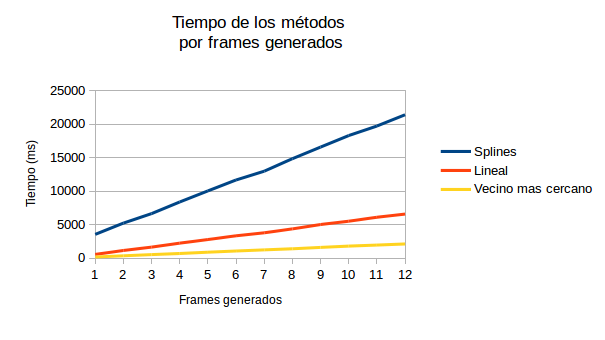
\includegraphics[scale= 0.6]{imagenes/aumentandoFramesToAdd.png}
  \end{center}
  \vspace{-10pt}
  \vspace{-10pt}
\end{wrapfigure}

Como vemos en el gráfico, el tiempo de procesamiento es lineal, esto es debido a que en cada iteración aumentamos la cantidad de frames a generar. Era de esperarse que un método como splines resultara ser el que más tarde en realizar su tarea, dado que realiza más operaciones que los otros métodos. \\

Por otro lado, realizamos una medición de tiempos con el mismo video, donde la cantidad de frames a generar es 1,   las dimensiones de los frames son fijas, y lo que variamos fue la cantidad de frames del video de entrada, aumentándolo de a 8 frames en cada medición. Para el video con movimiento, tomamos un segmento de un video largo tomando cada vez más frames, siempre desde el mismo frame original. Obtuvimos los siguientes resultados:


\begin{figure}[h!]
  \centering
    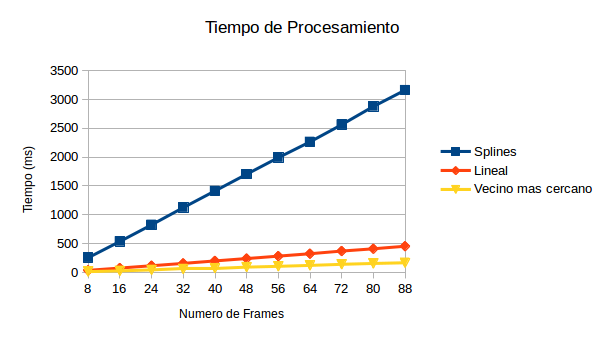
\includegraphics[scale= 0.8]{imagenes/aumentandoFramesMessi.png}
  \caption{Tiempo de Procesamiento agregando 1 frame aumentando la cantidad de frames originales}
\end{figure}

Los resultados que obtuvimos fueron lineales, como en el experimento anterior, con lo cual concluimos que la complejidad no depende únicamente de la cantidad de frames a generar, sino también de la cantidad de frames de entrada.\\


Intuitivamente el tiempo de procesamiento para cada método no debería variar si el video de prueba tiene gran movimiento o no, es decir, si hay mucha variacón del color de pixel entre frame y frame. Intuimos esto porque las operaciones que dependen del valor de un pixel son de tiempo constante (multiplicaciones, divisiones, sumas, restas y asignaciones). En particular, el video de prueba del experimento anterior, tenía una escena donde habia mucho movimiento, y esto no se reflejó en la medición temporal. \\

Por otro lado, tomamos los tiempo de procesamiento para un video del mismo ancho y largo que el video anterior, donde todos los frames eran blancos (todos los pixeles valen 255) tomando en cada medicion la misma cantidad de frames para poder ver efectivamente si los tiempos obtenidos eran menores, mayores o iguales. Los resultados obtenidos fueron muy parecidos al otro video, por lo que decidimos graficarlo tomando los tiempos del video con movimiento dividido el tiempo del video en blanco.

\begin{wrapfigure}{r}{0.6\textwidth}
  \vspace{-20pt}
  \begin{center}
    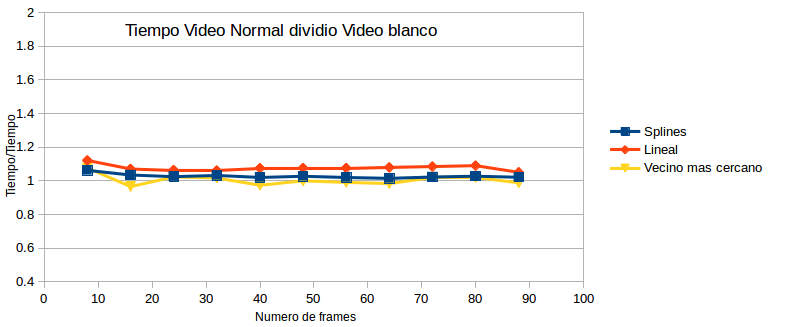
\includegraphics[scale= 0.6]{imagenes/aumentandoFramesMessiSobreWhite.png}
  \end{center}
  \vspace{-10pt}
  \vspace{-10pt}
\end{wrapfigure}

La mayor diferencia de tiempo entre ambos videos surgió en el método de splines. A pesar de no ser un tiempo significativamente distinto, creemos que la razón de que el tiempo sea ligeramente mayor en el video con movimiento radica en que los coeficientes de los polinomios obtenidos para el video en blanco son cero mientras que esto no sucede así para el otro video, haciendo que la evaluacion del polinomio sea más rápida.\\

Quedo por experimentar qué sucede con el tiempo cuando se varían ambos parámetros a la vez (frames generados y frames totales del video).



\subsection{Analisis de errores visuales por la aplicacion de los metodos}
\noindent Para esta sección utilizamos los siguiente videos:

$Gangnam Style:$ Video con cambios de cámara repentinos.

$Messi:$ Video con movimientos rápidos, sin cambios de cámara.

$Mario:$ Video del videojuego Super Mario Bros. Lo utilizamos por ser un video con movimientos rápidos, con el fin de poder observar diferencias visibles entre los métodos de 
interpolación.

$Tonalidad:$ Video de una suecesion de frames, donde cada frame es todo del mismo color, cambiando gradualmente de color, empezando desde el negro y terminando en el blanco. Lo utilizamos para ver las diferencias de colores generadas entre el método lineal y splines.\\

Primero utilizamos el video de $Gangnam Style$ para analizar los artifacts producidos por los cambios bruscos de cámara. El video tiene 3 cambios de cámara en 4 segundos. Ejecutamos los 3 métodos agregando 1 frame de por medio y comparamos las imágenes generadas justo en los cambios de cámara. Uno de ellos es el que se ve en la imágen. 

\newpage

%gangman:
\begin{figure}[h!]
  \centering
    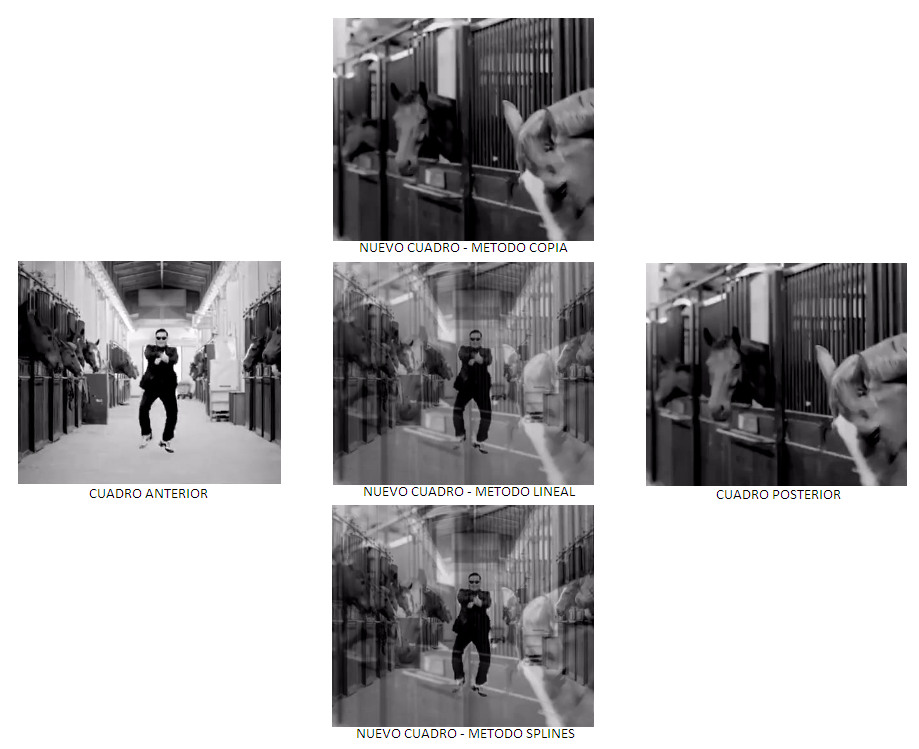
\includegraphics[scale= 0.5]{imagenes/gangman.png}
  \caption{Errores visuales por cambio de cámara}
\end{figure}


Como se puede ver en la Figura, el cambio brusco de camara genera frames intermedios no satisfactorios, donde parecería haber varios frames superpuestos y ligeramente corridos, mientras que con vecino más cercano no se ve este artifact, aunque obviamente se pierde cierta fluidez en el video en su totalidad.
Una posible manera de subsanar este artifact sería calculando la diferencia entre 2 frames, y si es más alta que cierto threshold, se considera que hubo un cambio brusco de camara, y en vez de calcular el polinomio interpolador entre esos 2 frames, se utiliza vecino más cercano.\\

Ahora queremos ver qué pasa cuando hay movimientos rápidos en alguna parte o en la totalidad del video, sin movimientos de cámara. Para esto utilizamos los videos de $Messi$ y de $Mario$. Para el video de $Messi$ interpolamos un único frame de por medio, y para el video de $Mario$, 5 frames. 

\newpage

\begin{figure}[h!]
  \centering
    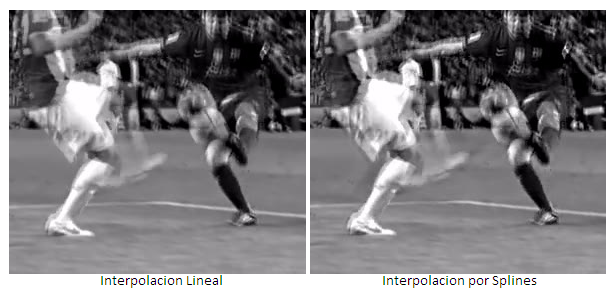
\includegraphics[scale= 0.5]{imagenes/messi.png}
  \caption{Errores visuales por rápidos movimientos}
\end{figure}


%messi:
No se pudieron apreciar diferencias significativas entre interpolacion lineal y splines. Ambos otorgan el mismo grado de fluidez al video. En el caso del vecino más cercano, cuando hay mucho movimiento, el video se ve muy cortado. Esto no se puede ver en las imágenes, pero en el video la diferencia es muy notoria.


\begin{figure}[h!]
  \centering
    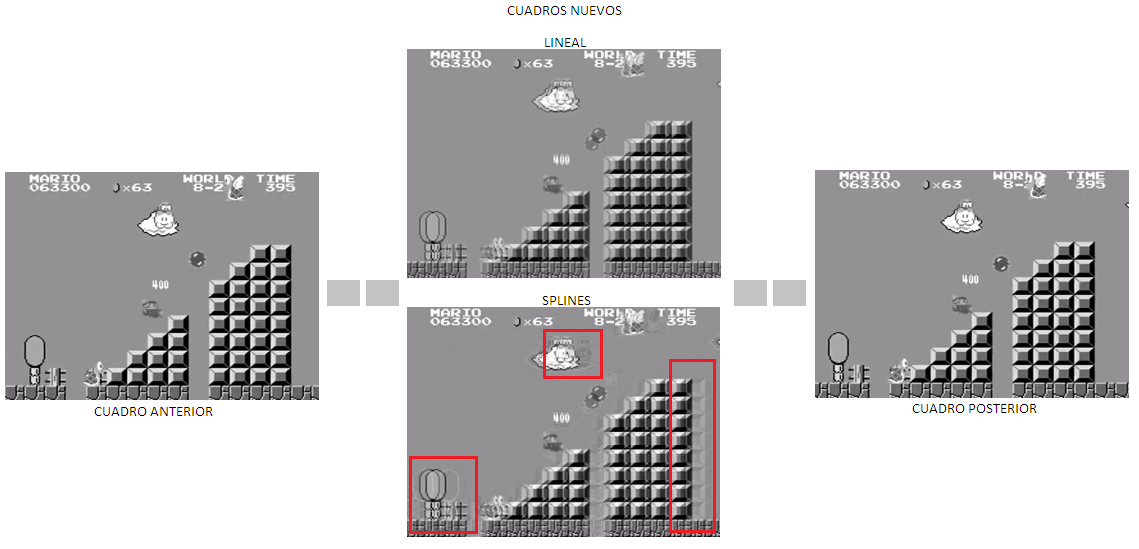
\includegraphics[scale= 0.587]{imagenes/mario.png}
  \caption{Errores visuales por rápidos movimientos}
\end{figure}


%mario:
En el video del $Mario$ al aplicar los metodos de interpolación, observamos diferencias claras entre ambos métodos. En la interpolación con splines, se puede ver que en los frames generados queda una suerte de blur que no está presente en los frames generados por interpolación lineal (zonas marcadas en rojo), lo que nos da a entender que en la interpolación por splines se esta utilizando mas información de los frames anteriores para generar el nuevo frame, otorgando visualmente una mayor fluidez al video.
Este efecto es más notorio mientras más frames se generan mediante interpolación. En el mismo video con 1 frame generado de por medio no se puede apreciar tanto esta diferencia.\\

También realizamos otro experimento con el video $Tonalidad$ (para el cual no agregamos imagenes ya que a simple vista no eran muy informativas de lo que estaba pasando) que consistió en un video generado por nosotros, el cual iba pasando por distintas tonalidades, empezando por el negro y aclarandose más hasta llegar al blanco. En este caso interpolación lineal y splines dieron diferentes, aunque fue una diferencia tan sutil que solo pudimos observarla comparando los valores de los píxeles con GIMP.\\

Tanto interpolación lineal como interpolación por splines dan resultados visualmente similares, salvo en el caso en que se generen muchos frames con interpolación.

\newpage
\subsection{Experimentación PSNR}

En esta sección analizamos las mediciones con el error cuadrático medio (ECM) y el Peak Signal to Noise Ratio (PSNR) y analizamos el impacto de los aspectos cualitativos de los vídeos en los métodos propuestos. \\

En el siguiente experimento, tomamos un video y le quitamos frames de a 1, para luego generarlos. Estudiamos como varía dicho índice comparando los frames originales que quitamos y los frames generados que los reemplazan. Utilizamos un video con cambios de cámara repentinos para poder ver como se comportan los métodos y ver el PSNR obtenido en esos cortes. Para esto, utilizamos un segmento del video $Gangnam Style$ que posee estas cualidades.
Los resultados que obtuvimos fueron los siguientes:


\begin{figure}[h!]
  \caption{Gráfico del PSNR comparando contra frames originales}
  \centering
    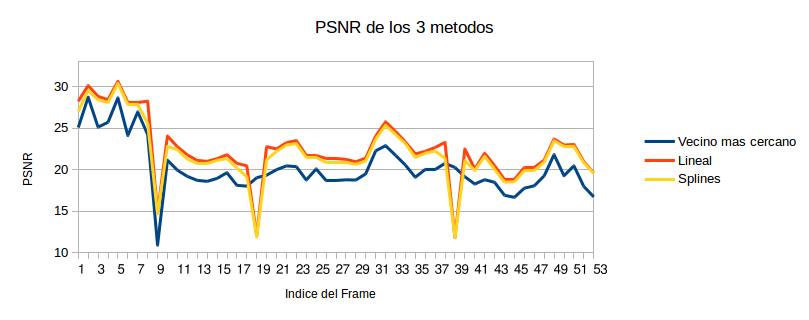
\includegraphics[scale=0.5]{imagenes/PSNRGangnam.png}
\end{figure}

Los picos inferiores del gráfico se corresponden con los frames donde ocurre un cambio de toma brusco. El pico más bajo corresponde al método del vecino más cercano, como esperabamos. Sin embargo, no sucede lo mismo con los otros dos picos. Esto se debe a que para esos frames, el algoritmo seleccinó los frames posteriores al cambio de toma, teniendo así una menor diferencia que los otros métodos.\\

Es interesante tambien ver qué sucede con los errores cuando agregamos muchos frames nuevos generados con los métodos. Usamos para este experimento un video con poco movimiento en los frames pero con movimientos rápidos ($Mario$). Aplicamos cada uno de los métodos generando 8 frames por cada 2 originales, y comparamos los frames generados con los frames que se quitaron, utilizando la medida de PSNR.

\begin{figure}[h!]
  \caption{Gráfico del PSNR comparando contra frames originales}
  \centering
    \includegraphics[scale=0.5]{imagenes/PSNR3metodosmario.png}
\end{figure}


Los picos que se ven en las tres funciones corresponden con frames nuevos que estaban más cerca de los frames originales es decir, se tiene mayor error al generar los frames que estan más alejados. Se corresponden tambien con los puntos de inflexión de los polinomios cúbicos que se usan para aproximarlos.\\

Tambien vemos que para este video en particular y cuando se generan muchos frames nuevos, el método de interpolación lineal funciona mejor si se mira cada imagen por separado. Sin embargo, cuando vemos el video generado por el método de splines los movimientos parecen ser mas fluidos y realistas. La medida de PSNR es más bien utilizada para medir la calidad de una imagen reconstruida por compresión y descompresión o para medir la calidad de una señal. Es por eso que no puede medir como queremos la calidad del movimiento.\\


Ahora vamos a analizar cual es la diferencia del error producido al agregar más o menos frames intermedios. En el experimento anterior agregamos una cantidad fija de frames y vimos como se comportaba el PSNR, ahora vamos a analizar la diferencia del error agregando 1 o 5 frames intermedios. Para esto, calculamos el PSNR del tercer frame de los 5 generados, y de los frames generados de a 1 que correspondían con los anteriores. 

\begin{figure}[h!]
  \caption{Gráfico del PSNR comparando contra frames originales con diferentes cantidades de frames agregados}
  \centering
    \includegraphics[scale=0.5401]{imagenes/PSNR1y5framesagregados.png}
\end{figure}

Como ya habíamos notado antes, la introducción de más frames entre cada par de frames originales aumenta el $"$ruido$"$ de la señal (que en este caso se puede interpretar como una imagen), lo cual se ve reflejado en una disminución en el PSNR, ya que aumenta el ECM debido al ruido. Sin embargo, no pudimos determinar la razón de los bajos valores de PSNR en los primeros frames generados.\\

Lo que quedo por experimentar es qué sucede cuando se realiza interpolación por splines variando el tamaño fijo de los bloques, y qué sucede cuando los tamaños del bloque son variables para una misma instancia.

%grafico de medicion de ecm con 
% \begin{wrapfigure}{r}{0.6\textwidth}
%   \vspace{-20pt}
%   \begin{center}
%     \includegraphics[scale= 0.6]{imagenes/.png}
%   \end{center}
%   \vspace{-10pt}
%   \vspace{-10pt}
% \end{wrapfigure}






